%        File: 2017-cnec.tex
%     Created: Fri Jul 21 09:00 AM 2017 E
% Last Change: Fri Jul 21 09:00 AM 2017 E
%
\documentclass[11pt,letterpaper]{article}
\usepackage[top=1.0in,bottom=1.0in,left=1.0in,right=1.0in]{geometry}
\usepackage{verbatim}
\usepackage{amssymb}
\usepackage{graphicx}
\usepackage{longtable}
\usepackage{amsfonts}
\usepackage{amsmath}
\usepackage[usenames]{color}
\usepackage[hidelinks]{hyperref}
\def\thesection       {\arabic{section}}
\def\thesubsection     {\thesection.\alph{subsection}}
\usepackage{xspace}
\newcommand{\Cyclus}{\textsc{Cyclus}\xspace}%
\usepackage[acronym,toc]{glossaries}
%\newacronym{<++>}{<++>}{<++>}
\newacronym[longplural={metric tons of heavy metal}]{MTHM}{MTHM}{metric ton of heavy metal}
\newacronym{ABM}{ABM}{agent-based modeling}
\newacronym{ACDIS}{ACDIS}{Program in Arms Control \& Domestic and International Security}
\newacronym{AHTR}{AHTR}{Advanced High Temperature Reactor}
\newacronym{ANDRA}{ANDRA}{Agence Nationale pour la gestion des D\'echets RAdioactifs, the French National Agency for Radioactive Waste Management}
\newacronym{ANL}{ANL}{Argonne National Laboratory}
\newacronym{API}{API}{application programming interface}
\newacronym{ARCH}{ARCH}{autoregressive conditional heteroskedastic}
\newacronym{ARE}{ARE}{Aircraft Reactor Experiment}
\newacronym{ARFC}{ARFC}{Advanced Reactors and Fuel Cycles}
\newacronym{ARMA}{ARMA}{autoregressive moving average}
\newacronym{ASME}{ASME}{American Society of Mechanical Engineers}
\newacronym{ATWS}{ATWS}{Anticipated Transient Without Scram}
\newacronym{BDBE}{BDBE}{Beyond Design Basis Event}
\newacronym{BIDS}{BIDS}{Berkeley Institute for Data Science}
\newacronym{BOL}{BOL}{Beginning-of-Life}
\newacronym{BSD}{BSD}{Berkeley Software Distribution}
\newacronym{CAFCA}{CAFCA}{ Code for Advanced Fuel Cycles Assessment }
\newacronym{CASL}{CASL}{Consortium for Advanced Simulation of Light Water Reactors}
\newacronym{CDTN}{CDTN}{Centro de Desenvolvimento da Tecnologia Nuclear}
\newacronym{CEA}{CEA}{Commissariat \`a l'\'Energie Atomique et aux \'Energies Alternatives}
\newacronym{CI}{CI}{continuous integration}
\newacronym{CNEC}{CNEC}{Consortium for Nonproliferation Enabling Capabilities}
\newacronym{CNEN}{CNEN}{Comiss\~{a}o Nacional de Energia Nuclear}
\newacronym{CNERG}{CNERG}{Computational Nuclear Engineering Research Group}
\newacronym{COSI}{COSI}{Commelini-Sicard}
\newacronym{COTS}{COTS}{commercial, off-the-shelf}
\newacronym{CSNF}{CSNF}{commercial spent nuclear fuel}
\newacronym{CTAH}{CTAHs}{Coiled Tube Air Heaters}
\newacronym{CUBIT}{CUBIT}{CUBIT Geometry and Mesh Generation Toolkit}
\newacronym{CURIE}{CURIE}{Centralized Used Fuel Resource for Information Exchange}
\newacronym{DAG}{DAG}{directed acyclic graph}
\newacronym{DANESS}{DANESS}{Dynamic Analysis of Nuclear Energy System Strategies}
\newacronym{DBE}{DBE}{Design Basis Event}
\newacronym{DESAE}{DESAE}{Dynamic Analysis of Nuclear Energy Systems Strategies}
\newacronym{DHS}{DHS}{Department of Homeland Security}
\newacronym{DOE}{DOE}{Department of Energy}
\newacronym{DRACS}{DRACS}{Direct Reactor Auxiliary Cooling System}
\newacronym{DRE}{DRE}{dynamic resource exchange}
\newacronym{DSNF}{DSNF}{DOE spent nuclear fuel}
\newacronym{DYMOND}{DYMOND}{Dynamic Model of Nuclear Development }
\newacronym{EBS}{EBS}{Engineered Barrier System}
\newacronym{EDZ}{EDZ}{Excavation Disturbed Zone}
\newacronym{EIA}{EIA}{U.S. Energy Information Administration}
\newacronym{EPA}{EPA}{Environmental Protection Agency}
\newacronym{EP}{EP}{Engineering Physics}
\newacronym{FCO}{FCO}{Fuel Cycle Options}
\newacronym{FCT}{FCT}{Fuel Cycle Technology}
\newacronym{FEHM}{FEHM}{Finite Element Heat and Mass Transfer}
\newacronym{FEPs}{FEPs}{Features, Events, and Processes}
\newacronym{FHR}{FHR}{Fluoride-Salt-Cooled High-Temperature Reactor}
\newacronym{FLiBe}{FLiBe}{Fluoride-Lithium-Beryllium}
\newacronym{GCAM}{GCAM}{Global Change Assessment Model}
\newacronym{GDSE}{GDSE}{Generic Disposal System Environment}
\newacronym{GDSM}{GDSM}{Generic Disposal System Model}
\newacronym{GENIUSv1}{GENIUSv1}{Global Evaluation of Nuclear Infrastructure Utilization Scenarios, Version 1}
\newacronym{GENIUSv2}{GENIUSv2}{Global Evaluation of Nuclear Infrastructure Utilization Scenarios, Version 2}
\newacronym{GENIUS}{GENIUS}{Global Evaluation of Nuclear Infrastructure Utilization Scenarios}
\newacronym{GPAM}{GPAM}{Generic Performance Assessment Model}
\newacronym{GRSAC}{GRSAC}{Graphite Reactor Severe Accident Code}
\newacronym{GUI}{GUI}{graphical user interface}
\newacronym{HLW}{HLW}{high level waste}
\newacronym{HPC}{HPC}{high-performance computing}
\newacronym{HTC}{HTC}{high-throughput computing}
\newacronym{HTGR}{HTGR}{High Temperature Gas-Cooled Reactor}
\newacronym{IAEA}{IAEA}{International Atomic Energy Agency}
\newacronym{IEMA}{IEMA}{Illinois Emergency Mangament Agency}
\newacronym{INL}{INL}{Idaho National Laboratory}
\newacronym{IPRR1}{IRP-R1}{Instituto de Pesquisas Radioativas Reator 1}
\newacronym{IRP}{IRP}{Integrated Research Project}
\newacronym{ISFSI}{ISFSI}{Independent Spent Fuel Storage Installation}
\newacronym{ISRG}{ISRG}{Independent Student Research Group}
\newacronym{JFNK}{JFNK}{Jacobian-Free Newton Krylov}
\newacronym{LANL}{LANL}{Los Alamos National Laboratory}
\newacronym{LBNL}{LBNL}{Lawrence Berkeley National Laboratory}
\newacronym{LCOE}{LCOE}{levelized cost of electricity}
\newacronym{LDRD}{LDRD}{laboratory directed research and development}
\newacronym{LFR}{LFR}{Lead-Cooled Fast Reactor}
\newacronym{LGPL}{LGPL}{Lesser GNU Public License}
\newacronym{LLNL}{LLNL}{Lawrence Livermore National Laboratory}
\newacronym{LMFBR}{LMFBR}{Liquid-Metal-cooled Fast Breeder Reactor}
\newacronym{LOFC}{LOFC}{Loss of Forced Cooling}
\newacronym{LOHS}{LOHS}{Loss of Heat Sink}
\newacronym{LOLA}{LOLA}{Loss of Large Area}
\newacronym{LP}{LP}{linear program}
\newacronym{LWR}{LWR}{Light Water Reactor}
\newacronym{MARKAL}{MARKAL}{MARKet and ALlocation}
\newacronym{MA}{MA}{minor actinide}
\newacronym{MCNP}{MCNP}{Monte Carlo N-Particle code}
\newacronym{MILP}{MILP}{mixed-integer linear program}
\newacronym{MIT}{MIT}{the Massachusetts Institute of Technology}
\newacronym{MOAB}{MOAB}{Mesh-Oriented datABase}
\newacronym{MOOSE}{MOOSE}{Multiphysics Object-Oriented Simulation Environment}
\newacronym{MOX}{MOX}{mixed oxide}
\newacronym{MSBR}{MSBR}{Molten Salt Breeder Reactor}
\newacronym{MSRE}{MSRE}{Molten Salt Reactor Experiment}
\newacronym{MSR}{MSR}{Molten Salt Reactor}
\newacronym{NAGRA}{NAGRA}{National Cooperative for the Disposal of Radioactive Waste}
\newacronym{NCSA}{NCSA}{National Center for Supercomputing Applications}
\newacronym{NEAMS}{NEAMS}{Nuclear Engineering Advanced Modeling and Simulation}
\newacronym{NEUP}{NEUP}{Nuclear Energy University Programs}
\newacronym{NFCSim}{NFCSim}{Nuclear Fuel Cycle Simulator}
\newacronym{NFC}{NFC}{Nuclear Fuel Cycle}
\newacronym{NGNP}{NGNP}{Next Generation Nuclear Plant}
\newacronym{NMWPC}{NMWPC}{Nuclear MW Per Capita}
\newacronym{NNSA}{NNSA}{National Nuclear Security Administration}
\newacronym{NPRE}{NPRE}{Department of Nuclear, Plasma, and Radiological Engineering}
\newacronym{NQA1}{NQA-1}{Nuclear Quality Assurance - 1}
\newacronym{NRC}{NRC}{Nuclear Regulatory Commission}
\newacronym{NSF}{NSF}{National Science Foundation}
\newacronym{NSSC}{NSSC}{Nuclear Science and Security Consortium}
\newacronym{NUWASTE}{NUWASTE}{Nuclear Waste Assessment System for Technical Evaluation}
\newacronym{NWF}{NWF}{Nuclear Waste Fund}
\newacronym{NWTRB}{NWTRB}{Nuclear Waste Technical Review Board}
\newacronym{OCRWM}{OCRWM}{Office of Civilian Radioactive Waste Management}
\newacronym{ORION}{ORION}{ORION}
\newacronym{ORNL}{ORNL}{Oak Ridge National Laboratory}
\newacronym{PARCS}{PARCS}{Purdue Advanced Reactor Core Simulator}
\newacronym{PBAHTR}{PB-AHTR}{Pebble Bed Advanced High Temperature Reactor}
\newacronym{PBFHR}{PB-FHR}{Pebble-Bed Fluoride-Salt-Cooled High-Temperature Reactor}
\newacronym{PEI}{PEI}{Peak Environmental Impact}
\newacronym{PH}{PRONGHORN}{PRONGHORN}
\newacronym{PI}{PI}{Principal Investigator}
\newacronym{PRKE}{PRKE}{Point Reactor Kinetics Equations}
\newacronym{PSPG}{PSPG}{Pressure-Stabilizing/Petrov-Galerkin}
\newacronym{PWAR}{PWAR}{Pratt and Whitney Aircraft Reactor}
\newacronym{PWR}{PWR}{Pressurized Water Reactor}
\newacronym{PyNE}{PyNE}{Python toolkit for Nuclear Engineering}
\newacronym{PyRK}{PyRK}{Python for Reactor Kinetics}
\newacronym{QA}{QA}{quality assurance}
\newacronym{RDD}{RD\&D}{Research Development and Demonstration}
\newacronym{RD}{R\&D}{Research and Development}
\newacronym{RELAP}{RELAP}{Reactor Excursion and Leak Analysis Program}
\newacronym{RIA}{RIA}{Reactivity Insertion Accident}
\newacronym{RIF}{RIF}{Region-Institution-Facility}
\newacronym{SAM}{SAM}{Simulation and Modeling}
\newacronym{SFR}{SFR}{Sodium-Cooled Fast Reactor}
\newacronym{SINDAG}{SINDA{\textbackslash}G}{Systems Improved Numerical Differencing Analyzer $\backslash$ Gaski}
\newacronym{SKB}{SKB}{Svensk K\"{a}rnbr\"{a}nslehantering AB}
\newacronym{SNF}{SNF}{spent nuclear fuel}
\newacronym{SNL}{SNL}{Sandia National Laboratory}
\newacronym{SNM}{SNM}{Special Nuclear Material}
\newacronym{STC}{STC}{specific temperature change}
\newacronym{SUPG}{SUPG}{Streamline-Upwind/Petrov-Galerkin}
\newacronym{SWF}{SWF}{Separations and Waste Forms}
\newacronym{SWU}{SWU}{Separative Work Unit}
\newacronym{SandO}{S\&O}{Signatures and Observables}
\newacronym{TRIGA}{TRIGA}{Training Research Isotope General Atomic}
\newacronym{TRISO}{TRISO}{Tristructural Isotropic}
\newacronym{TSM}{TSM}{Total System Model}
\newacronym{TSPA}{TSPA}{Total System Performance Assessment for the Yucca Mountain License Application}
\newacronym{UFD}{UFD}{Used Fuel Disposition}
\newacronym{UML}{UML}{Unified Modeling Language}
\newacronym{UOX}{UOX}{uranium oxide}
\newacronym{UQ}{UQ}{uncertainty quantification}
\newacronym{US}{US}{United States}
\newacronym{UW}{UW}{University of Wisconsin}
\newacronym{VISION}{VISION}{the Verifiable Fuel Cycle Simulation Model}
\newacronym{VV}{V\&V}{verification and validation}
\newacronym{WIPP}{WIPP}{Waste Isolation Pilot Plant}
\newacronym{YMR}{YMR}{Yucca Mountain Repository Site}

\makeglossaries
\date{}

\author{Kathryn Huff\\
        Blue Waters Assistant Professor\\
        Department of Nuclear, Plasma, and Radiological Engineering\\
        University of Illinois at Urbana-Champaign\\
         \href{mailto:kdhuff@illinois.edu}{\texttt{kdhuff@illinois.edu}}}

         \title{\vspace{-1in}Fuel Cycle Simulation Capability for Signatures and Observables}
\begin{document}
\maketitle
\section{Project Description}

Nuclear power plants themselves are typically considered a lower proliferation 
risk than other fuel cycle facilities, particularly those which produce or 
recycle fuel 
\cite{national_academy_of_sciences_americas_2009,national_research_council_proliferation_2012}. Accordingly, dynamic fuel cycle 
facility modeling is essential to assessment of proliferation risk, 
safeguardability, and material accountancy robustness. 

Students will develop fuel cycle facility models, or \emph{archetypes}, for use 
with the \Cyclus agent-based fuel cycle simulator \cite{huff_fundamental_2016}. 
These dynamically loadable, C++ shared-object libraries will capture material 
streams within myriad front-end and back-end fuel cycle facilities in support 
of nonproliferation-focused analysis.  Specifically, one graduate student and up 
to four undergraduate students will improve existing enrichment, reactor, and 
reprocessing facility models to better capture material flows which impact 
material accountancy or qualify as observable signatures.  

Recent work by McGarry et al. \cite{mcgarry_mbmore_2017} has extended the 
\Cyclus fuel cycle simulator \cite{huff_fundamental_2016} ecosystem to include 
archetypes dedicated to modeling non-deterministic, nonproliferation-related 
treaty verification behavior in a simple enrichment facility. This proposal 
will build upon that work.  The proposed effort will significantly improve the 
fidelity of these capabilities for characterizing \gls{SNM} signature and 
diversion detection sensitivity \cite{mcgarry_mbmore_2017}.  \emph{Archetype} 
fidelity in this sense refers to the ability to capture the dominant physics of 
the particular facility technology at levels of detail appropriate to influence 
conclusions.

Student effort will emphasize conventional fuel cycle facilities in support of 
\Cyclus use cases focused on `shadow' fuel cycles, diversion detection, and 
signature disambiguation (e.g.
\cite{boyer_developing_2014}, \cite{hou_diversion_2016} 
\cite{rossi_application_2015}, and \cite{yilmaz_online_2016}).  However, students will also explore potential future technologies and advanced fuel cycles such as \gls{MSR} online fuel reprocessing concepts, laser enrichment, etc.  The resulting simulation library will enable users of the \Cyclus simulator, both scientists and students, to conduct more sophisticated dynamic simulations relevant to non-proliferation (e.g.  systems assessment for safeguardability as in \cite{borrelli_approaches_2017}.  Specifically, increased mass flow fidelity at the sub-facility level will enable users to answer novel questions concerning intrinsic features of fuel cycle facility mass flows.

\section{Relevance to CNEC}
This work will improve existing capabilities for characterization of facilities
which process \gls{SNM}. Additionally, the research process will train 
undergraduate and graduate students in modeling and simulation of the nuclear 
fuel cycle.  Additionally, emphasis on student
technical modeling and simulation skills will benefit from the experience of the 
\gls{PI} in the area of scientific computing best practices 
\cite{scopatz_effective_2015,wilson_best_2014,huff_lessons_2017,huff_case_2017}.

Application of the proposed capabilities to signature detection and diversion 
sensitivity is relevant to the \gls{CNEC} \gls{SandO} thrust area goals.  
Simultaneously, this work has a core focus on modeling and simulation that is 
quite relevant to the \gls{CNEC} \gls{SAM} thrust area.  

Finally, through direct collaboration with \Cyclus ecosystem community members 
at the national laboratories, including \gls{ORNL} and \gls{PNNL} in particular, students will be enabled to pursue internships with the national laboratories.

\section{Tasks and Deliverables}

At least eight new \Cyclus \emph{archetypes} will be developed according to the 
schedule described in Figure \ref{fig:milestones}.  These \emph{archetypes} 
will be used to demonstrate improved fidelity of \Cyclus analysis related to 
detection of signatures indicative of \gls{SNM} or \gls{SNM} diversion. 
All \emph{archetypes} developed in this work will be accompanied by sufficient 
documentation, testing, and integration with the simulator to enable reuse by 
other fuel cycle analysts\footnote{In accordance with the \Cyclus ecosystem, 
the products of this work will be BSD-3 licensed.}.


\begin{figure}[htbp!]
        \begin{center}
                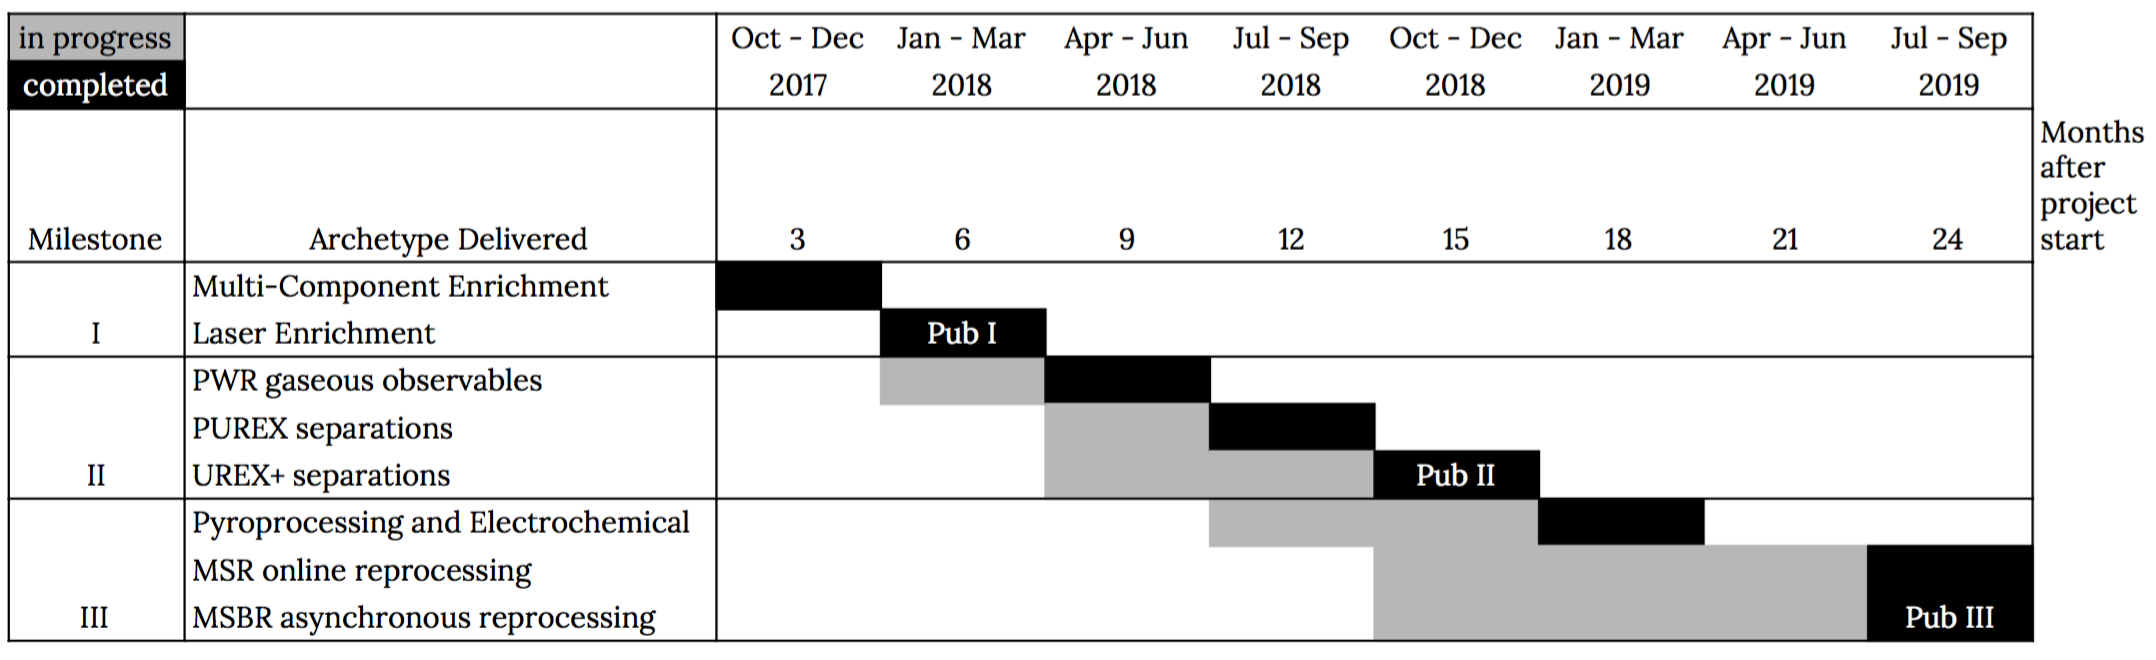
\includegraphics[width=\textwidth]{milestones.png}
        \end{center}
        \caption{The development of \Cyclus archetypes, one per quarter, is 
                organized into chronological and thematic milestones. Each 
                milestone will be  accompanied by a publication demonstrating 
        analytic use cases enabled by the new archetypes.} 
        \label{fig:milestones}
\end{figure}

\paragraph{Milestone I} will focus on signatures and observables related to 
enrichment facilities, both conventional (gaseous centrifuge cascades) and 
advanced (laser isotopic separation). 

\paragraph{Milestone II} will focus on model fidelity that enables the analyst 
to potentially disambiguate civilian power generation signatures from those 
generated by separations and reprocessing activities. This milestone will 
accordingly include detailed PUREX and UREX+ separations models as well as 
fidelity improvements to existing \gls{PWR} models. Detail in all of these 
facility \emph{archetypes} will capture release streams of disambiguating 
isotopes such as $^{85}Kr$, $^{135}Xe$, and $^{133}Xe$ 
\cite{kalinowski_isotopic_2006,kemp_environmental_2016}.

\paragraph{Milestone III} will explore development of reprocessing models 
appropriate for advanced reactor types. Specifically, this work will look at 
the unique case of \glspl{MSR} which have recently gained renewed interest. 
Both online and asynchronous \gls{MSR} reprocessing strategies will be modeled. 
Again these models will be implemented at a level of fidelity which captures 
isotope releases with environmentally detectable signatures. 


\bibliographystyle{ieeetr}
\bibliography{2017-cnec-signatures}


\pagebreak
\section*{Budget}
The budget assumes a project duration of two years.  
As requested, the budget for this project is attached in Excel format.
This work will require the 
50\% effort of one graduate student at the University of Illinois College of 
Engineering Research Assistant rate and 50\% effort of one hourly undergraduate 
at a rate of \$10 per hour.  It will also require one month of \gls{PI} effort 
per year. If a suitable graduate student cannot be identified in the 2017-2018 
academic year, the work of the graduate student can be conducted for similar 
cost by four undergraduate students, each working 20 hours per week.  

Publication costs assume one 20 page 
article per year at a cost of \$50 per page.  Finally, this work will require 
travel funding for the graduate student and the \gls{PI} to present their work in a conference setting annually.  


\end{document}


